\section{Introduction}\label{sec:intro}

The Hodge conjecture asks that every rational cohomology class of type $(p,p)$ on a smooth complex projective variety be a rational combination of classes of algebraic subvarieties.\footnote{An earlier preprint of the authors, \emph{Relative secant cycles and Hodge classes}, Preprints.org (2026), \nolinkurl{doi:10.20944/preprints202602.0462.v5} \cite{BB26}, claimed a proof of the Hodge conjecture that does not hold, and the present paper replaces it. The secant variety $\mathrm{Sec}^{n}(A^{\vee})$ contains $A^{\vee}$, so the cycle $\Sigma\cap A^{\vee}$ of its Definition~3 is $A^{\vee}$ itself, whose Fourier--Mukai transform is a skyscraper sheaf with no component in degree $2n$, contrary to its Lemma~4. The Weil classes span a $2$-dimensional space on which $K^{\times}$ acts by $\tau\mapsto\tau^{2n}$, while $\eta^{n}$ has character $N(\tau)^{n}$, contrary to its Propositions~1 and~2. Its general case (Theorem~12) applies the Kuga--Satake construction outside Hodge structures of K3 type and assumes the Kuga--Satake correspondence algebraic, which is open. Section~\ref{sec:earlier} lists every point at which that preprint fails.} Hodge raised it in 1950 \cite{Hod50}; Lefschetz had proved it for divisors \cite{Lef24}. It is known in a scattered family of cases and open in general. This paper does three things. It proves that the conjecture is equivalent to two statements about abelian varieties. It proves that the locus on which either statement is known has the same shape in every family, dense and either everything or meagre, so that each statement asks that algebraicity propagate from a dense set of special points to the whole family. And it builds, at the first class each statement has to reach, an explicit object, proves what that object does, and names the step at which it stops. The conjecture does not close here. What the paper adds is a complete account of where the two remaining statements live, two new theorems on real multiplication, by $\QQ(\sqrt6)$ on K3 surfaces and by the cyclic cubic fields $\QQ(\zeta_{7})^{+}$ and $\QQ(\zeta_{9})^{+}$ on the surfaces of Mumford type, the second of which closes the first two cases of the frontier of \cite{BMB26}, and three constructions carried to the point where the next step is a single stated question. Figure~\ref{fig:roadmap} draws this plan.

\begin{figure*}[t]
\centering
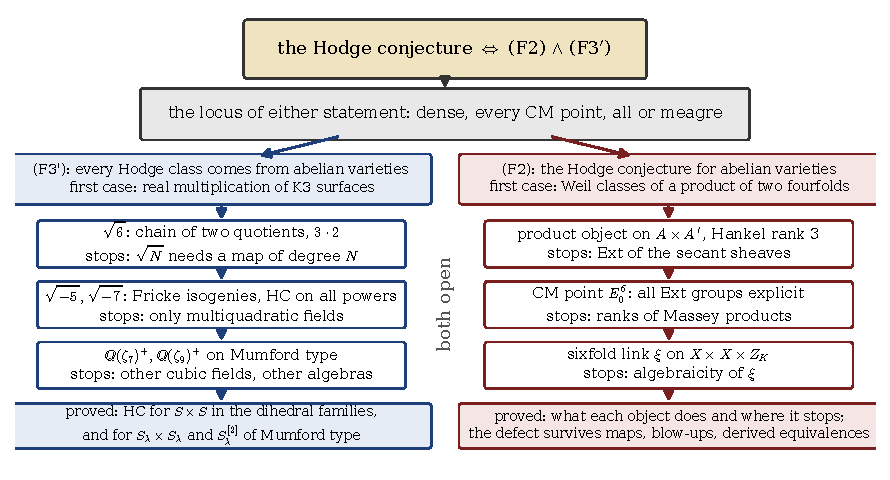
\includegraphics[width=0.96\textwidth]{figures/fig_roadmap}
\caption{The plan of the paper. The conjecture is equivalent to \Fii{} and \Fiii{} (Theorem~\ref{thm:intro-reduction}, Proposition~\ref{prop:minimal}); the locus of either statement is dense, contains every CM point and is all or meagre (Section~\ref{sec:loci}). For \Fiii{} the first class is the real multiplication of K3 surfaces: the chain of quotients for $\sqrt6$ (Theorem~\ref{thm:sqrt6}), the Fricke isogenies for $\sqrt5$ and $\sqrt7$ (Theorem~\ref{thm:fricke}), the cyclic cubic fields on the surfaces of Mumford type (Theorem~\ref{thm:zeta9}), and the steps at which each stops (Propositions~\ref{prop:structure} and~\ref{prop:cubicstop}). For \Fii{} the first class is the Weil classes of a product of two fourfolds: the product object (Theorem~\ref{thm:product}, stopping at Proposition~\ref{prop:convolution}), the point of complex multiplication (Lemma~\ref{lem:cmext}, stopping at Proposition~\ref{prop:twostep}) and the sixfold link (Theorem~\ref{thm:link}, stopping at Section~\ref{ssec:f2stop2}); the defect survives the operations of Proposition~\ref{prop:surgery}.}
\label{fig:roadmap}
\end{figure*}

\subsection{The two statements}

Write $\HC$ for the Hodge conjecture for all smooth complex projective varieties and $\AB$ for its restriction to abelian varieties. For a smooth projective variety $X$ and an integer $p$ let $\Hdg^{p}(X)$ be the Hodge classes of degree $2p$, and let $\Ab^{p}(X)\subseteq\Hdg^{p}(X)$ be the span of the classes $\Gamma_{*}\gamma$, where $B$ runs over the complex abelian varieties (the point included), $\gamma$ over the Hodge classes on $B$, and $\Gamma$ over the algebraic correspondences from $B$ to $X$. The two statements are
\begin{itemize}[leftmargin=2.4em,itemsep=2pt]
\item[\Fii] every Hodge class on every complex abelian variety is algebraic, in the form in which it first appears in the closure computation of \cite{BMB26}: the Hodge classes of the smallest known instance, the exceptional classes on the square of a Mumford fourfold, are algebraic together with everything that can be built from them;
\item[\Fiii] $\Hdg^{p}(X)=\Ab^{p}(X)$ for every $X$ and every $p$: every Hodge class is algebraic modulo the images, under algebraic correspondences, of Hodge classes of abelian varieties.
\end{itemize}

\begin{theorem}[Reduction]\label{thm:intro-reduction}
$\HC$ holds if and only if \Fii{} and \Fiii{} both hold; \Fii{} is equivalent to $\AB$, and \Fiii{} holds on every abelian variety, on every variety dominated by a product of curves or by an abelian variety, and on every variety in degrees $2p$ with $p\in\{0,1,\dim X-1,\dim X\}$.
\end{theorem}

The content of the theorem is in the second sentence: \Fii{} is not a special case of the conjecture for abelian varieties but the whole of it, carried by its hardest classes, and \Fiii{} is exactly what the conjecture asks of the part of the cohomology of $X$ that no abelian variety reaches. Section~\ref{sec:reduction} proves it and places the two statements in the closure graph of the known reductions, with the Lefschetz standard conjecture, Andr\'e's motivated classes and the variational Hodge conjecture as the other nodes (Fig.~\ref{fig:graph}).

\subsection{The shape of the known locus}

For a smooth projective family $\pi\colon\mathcal{X}\to S$ and a flat Hodge class $\xi$ let $\Sigma(\xi)\subseteq S$ be the set of points at which $\xi$ is algebraic.

\begin{theorem}[Dichotomy and propagation]\label{thm:intro-loci}
\leavevmode
\begin{enumerate}[label=\textup{(\roman*)},leftmargin=2.4em,itemsep=2pt]
\item $\Sigma(\xi)$ is a countable union of Zariski closed subsets of $S$, and either $\Sigma(\xi)=S$ or $\Sigma(\xi)$ is meagre.
\item \Fii{} holds if and only if, for every polarised abelian scheme and every flat Hodge class $\xi$, algebraicity of $\xi$ at one point of complex multiplication forces $\Sigma(\xi)=S$.
\item For the Weil classes of every CM field, every $n\ge2$ and every discriminant, $\Sigma(\xi)$ contains an explicit point of complex multiplication and is dense.
\item \Fiii{} holds for $X$ in degree $2p$ if and only if a Hodge complement of the abelian part of $H^{2p}(X,\QQ)$ carries no nonzero Hodge class.
\end{enumerate}
\end{theorem}

So both statements have the same form. There is a dense set of points, the points of complex multiplication, at which the class is known to be algebraic by explicit cycles; the locus of algebraicity is a countable union of closed strata; and the conjecture is the statement that this union is not meagre. Figure~\ref{fig:locus} draws it. Section~\ref{sec:loci} proves the theorem, after \cite{BMB26}, whose argument we rewrite in the generality needed here.

\subsection{Constructions at the first class}

The rest of the paper is constructive. At each statement we go to the first class that is not known and build the object that would make it algebraic.

At \Fiii{} the first class lives on powers of a K3 surface $S$ with real multiplication: the transcendental lattice $T(S)_{\QQ}$ is a vector space over a totally real field $E=\End_{\Hdg}T(S)_{\QQ}$, and the elements of $E$ are Hodge classes on $S\times S$. Section~\ref{sec:f3prime} proves:

\begin{theorem}[Chains of symplectic quotients]\label{thm:intro-chain}
Let $S$ be a projective K3 surface and $e\in E$ with $e^{2}=n\in\QQ_{>0}$. If there is a chain of projective K3 surfaces $S=S_{0},S_{1},\dots,S_{r}$ joined by dominant rational maps or rational Hodge isometries whose degrees multiply to $n$ modulo squares, then $e$ is algebraic on $S\times S$. In particular, for every projective K3 surface $S$ with $\QQ(\sqrt6)\subseteq E$ whose transcendental space embeds in the invariant lattice of a symplectic automorphism of order three, the real multiplication by $\sqrt6$ is algebraic, the Hodge conjecture holds for $S\times S$ and $S^{[2]}$, and such surfaces form two-dimensional families whose very general member has $E=\QQ(\sqrt6)$ exactly.
\end{theorem}

Varesco \cite{Var23} proved the case of a single quotient by a symplectic automorphism of prime order, which gives $\sqrt2$ and $\sqrt3$; van Geemen and Sch\"utt \cite{vGS25} reach $\sqrt2,\sqrt3,\sqrt7$ through rational self-maps. The chain adds $\sqrt6$, the first composite value, with the lattice condition made explicit. A second construction in Section~\ref{sec:f3prime} starts from the universal elliptic curve over the modular curves $X_{0}(5)$ and $X_{0}(7)$: the Fricke involution lifts to an isogeny of degree $5$ or $7$ between the elliptic K3 surface over the base and the one over its image, and on the quadratic twists of the two surfaces by the same pair of parameters it becomes a rational map of that degree between two K3 surfaces of the same family. Theorem~\ref{thm:fricke} shows that the very general member of each family has Picard number $16$ and real multiplication by $\QQ(\sqrt5)$ or $\QQ(\sqrt7)$, that the multiplication is the pushforward of the isogeny and so is algebraic, and that the Hodge conjecture holds for the square of every member. The method also shows exactly why it stops. Proposition~\ref{prop:structure} describes the action of an arbitrary correspondence on the transcendental lattice: every component whose resolution has geometric genus at most one acts as a similarity, with multiplier the product of the degrees of its two projections, a composite returning to $S$ is an element of $E$ with rational square, and these span only the multiquadratic subfield of $E$; a correspondence reaching anything else has a component of geometric genus at least two and transcendental rank at least twice that of $S$. Proposition~\ref{prop:hecke} shows that the correspondences cut out of finite groups acting on covers of $S$, which include the graphs of the dihedral families of \cite{vGS25}, produce only abelian fields, and Corollary~\ref{cor:dihedral} draws the consequence that the Hodge conjecture holds on $X\times X$ for every member of those families. For the cubic field of the frontier case of \cite{BMB26} the multiquadratic subfield is $\QQ$ and the field is not cyclic in general, so both constructions are blind to it. A third is not. For the two cyclic cubic fields $F=\QQ(\zeta_{7})^{+}$ and $\QQ(\zeta_{9})^{+}$ the quaternion algebra over $F$ ramified at exactly two real places is the even Clifford algebra of a two-dimensional dihedral family of K3 surfaces of Picard number ten, and weak approximation in the norm-one group of that algebra moves the period of the surface of Mumford type into the image of the family; Theorem~\ref{thm:zeta9} makes the real multiplication by $F$ algebraic there, through Buskin's theorem, and proves the Hodge conjecture for $S_{\lambda}\times S_{\lambda}$ and for the Hilbert square of $S_{\lambda}$. Proposition~\ref{prop:cubicstop} then says exactly what the mechanism cannot reach: the algebras over these fields ramified at finite places, which no rank-twelve family carries, the cyclic cubic fields of larger conductor, which no finite group acting on $\mathbb{P}^{1}$ produces, and the fields with Galois group $S_{3}$. The frontier is every pair of a cubic field and a quaternion algebra other than these two.

At \Fii{} the first class is a Weil class of a very general abelian $2n$-fold of Weil type with $n\ge3$, or the exceptional class of a Mumford fourfold. For the Weil classes the tool is the polarised semiregularity criterion of \cite{BMB26}: a perfect complex $\mathcal{E}$ whose Chern character is a nonzero multiple of a Weil class plus a polynomial in the polarisation, with $\dim\Ext^{2}(\mathcal{E},\mathcal{E})$ equal to the lower bound $r(\gamma)=(4+\rho)n^{2}-2n$, makes the Weil classes algebraic on every member with full Hodge group. Section~\ref{sec:f2} proves:

\begin{theorem}[The product object]\label{thm:intro-product}
Let $A$, $A'$ be very general polarised abelian varieties of Weil type for the same imaginary quadratic field, of dimensions $2m$, $2m'$, with algebraic Weil classes, and let $n=m+m'$. There is a perfect complex $\mathcal{E}$ on $A\times A'$, a direct sum with shifts of exterior products of secant sheaves and powers of the polarisations, whose Chern character has the polarised shape with Hankel rank $\rho=3$, so that $r(\gamma)=7n^{2}-2n$, and whose first-order Hodge locus is the whole tangent space of the polarised Weil family. Every such direct sum has $\dim\Ext^{2}(\mathcal{E},\mathcal{E})>r(\gamma)$, and its semiregularity map is not injective. The criterion can therefore be met at a product point only by a convolution of these pieces with nonzero differentials.
\end{theorem}

For the exceptional classes of a Mumford fourfold $X$ we replace the K3 surface that carries their transcendental part in \cite{BMB26} by an abelian sixfold $Z_{K}$ over the same Shimura curve, so that the whole problem stays inside abelian varieties.

\begin{theorem}[The sixfold link]\label{thm:intro-link}
Let $X$ be a Mumford fourfold with cubic field $F$, let $K=F(\sqrt{-\delta})$ be a CM extension inside the quaternion algebra, and let $Z_{K}$ be the abelian sixfold of Shimura type attached to $K$ over the Shimura curve of $X$. The Hodge classes in $H^{1}(X)\otimes H^{1}(X)\otimes H^{2}(Z_{K})$ that identify the two copies of the nine-dimensional representation $T$ form a line over $F$, spanned by a class $\xi$. If $\xi$ is algebraic and $K$ contains no imaginary quadratic field, the exceptional classes of $X\times X$ are algebraic, and so is every Hodge class on every power of $X$. Conversely the algebraicity of $\xi$ is equivalent to the algebraicity of the exceptional classes together with one algebraic link from $Z_{K}$ to a power of $X$.
\end{theorem}

Neither theorem closes \Fii{}. Section~\ref{sec:f2} says what each needs next: for Theorem~\ref{thm:intro-product} the Ext algebra of Markman's secant sheaves, which no published result computes at a very general point, and which Lemma~\ref{lem:cmext} computes at the point $E_{0}^{6}$ of complex multiplication, where Proposition~\ref{prop:twostep} leaves the ranks of the Massey products of length at least three as the one open quantity; for Theorem~\ref{thm:intro-link} the algebraicity of one class in a mixed K\"unneth component of an abelian fourteenfold, which no known theorem produces even at the points of complex multiplication.

\subsection{What is proved and what is not}

Table~\ref{tab:status} in Section~\ref{sec:status} lists every statement of the paper with its status. The reduction, the dichotomy, Theorem~\ref{thm:intro-chain} and the two constructions are proved. \Fii{} and \Fiii{} are open, and with them the conjecture. We state this at the outset because the earlier preprint named in the footnote did not, and because the value of the constructions lies in the precision of the question each one leaves.

Appendix~\ref{app:checks} describes the machine checks: a Lean~4 file that verifies the closure graph, the character computation behind the footnote and the dimension counts of Section~\ref{sec:f2}, with no axiom beyond propositional extensionality; the Lean certificate of \cite{BMB26} on which the reduction rests; and programs in Python, Julia, C, C\texttt{++} and shell that recompute every finite quantity used in the proofs. No statement of the paper rests on a computation.
